\documentclass{article}

% preambulo:
\usepackage[utf8]{inputenc}
% caracteres utf8 (tildes, enie) sin tener que usar comandos

\usepackage[spanish, es-tabla, es-nodecimaldot]{babel} 
% texto automatico en espaniol
% "tabla" en vez de "cuadro"
% no reemplaza puntos decimales por comas

%% NO AGREGAR PAQUETES ANTES DE ESTO, ES IMPORTANTE QUE BABEL ESTE PRIMERO

%%%%%%%%%%%%%%%%%%%%%%%%%%%%%%%%%
%% PAQUETES EXTRA %%%%%%%%%%%%%%%
%%%%%%%%%%%%%%%%%%%%%%%%%%%%%%%%%

\usepackage{subfiles}

%nuevo
\usepackage[notransparent]{svg}
%

\usepackage{amsmath} % PAQUETES DE MATEMATICA
\usepackage{amsfonts}
\usepackage{amssymb}

%puse esta cosa nueva---
\usepackage{csvsimple}

%-----
\usepackage{steinmetz} % comando \phase{}
\usepackage{units} % permite usar nicefrac
\usepackage{graphicx} % importar imagenes
\usepackage{float} % posicion H para floats
\usepackage[colorinlistoftodos]{todonotes}


\usepackage[a4paper, total={6in, 8in}]{geometry} 
% margenes correctos en subarchivos

\setlength{\parindent}{10pt}			%cuanta sangria al principio de un parrafo
\usepackage{indentfirst}				%pone sangria al primer parrafo de una seccion

\usepackage{listings}

\usepackage{color}

\definecolor{codegreen}{rgb}{0,0.6,0}
\definecolor{codegray}{rgb}{0.5,0.5,0.5}
\definecolor{codepurple}{rgb}{0.58,0,0.82}
\definecolor{backcolour}{rgb}{0.95,0.95,0.92}
 
\lstdefinestyle{mystyle}{
    backgroundcolor=\color{backcolour},   
    commentstyle=\color{codegreen},
    keywordstyle=\color{magenta},
    numberstyle=\tiny\color{codegray},
    stringstyle=\color{codepurple},
    basicstyle=\footnotesize,
    breakatwhitespace=false,         
    breaklines=true,                 
    captionpos=b,                    
    keepspaces=true,                 
    numbers=left,                    
    numbersep=5pt,                  
    showspaces=false,                
    showstringspaces=false,
    showtabs=false,                  
    tabsize=2
}
 
\lstset{style=mystyle}

%%%%%%%%%%%%%%%%%%%%%%%%%%%%%%%%%%%%%%%%%%%%%%%%%%%%%%%%%%%
%% NO AGREGAR PAQUETES DESPUES DE ESTO, ES IMPORTANTE QUE HYPERREF ESTE ULTIMO
\usepackage[hidelinks]{hyperref} % hipervinculos sin cajitas rojas
\usepackage{bm}


\begin{document}

\newgeometry{} % margenes default para la caratula
% caratula:
\begin{titlepage}
\newcommand{\HRule}{\rule{\linewidth}{0.5mm}}
\center
\mbox{\textsc{\LARGE \bfseries {Instituto Tecnol\'ogico de Buenos Aires}}}\\[1.5cm]
\textsc{\Large 22.85 - Sistemas de Control}\\[0.5cm]


\HRule \\[0.6cm]
{ \Huge \bfseries Trabajo de Laboratorio N$^{\circ}$2: Realimentación Lineal de estados}\\[0.4cm] % Title of your document
\HRule \\[1.5cm]


{\large

\emph{Grupo 1}\\
\vspace{3px}

\begin{tabular}{lr} 	
\textsc{M\'aspero}, Martina  & 57120 \\
\textsc{Mestanza}, Joaqu\'in Mat\'ias  & 58288 \\
\textsc{Nowik}, Ariel Santiago  & 58309 \\
\textsc{Panaggio Venerandi}, Guido Martin  & 56214 \\
\textsc{Parra}, Roc\'io  & 57669 \\
\textsc{Regueira}, Marcelo Daniel  & 58300 \\

\end{tabular}

\vspace{20px}

\emph{Profesor}\\
\vspace{3px}
\textsc{Nasini}, V\'ictor Gustavo\\ 	
\vspace{100px}

\begin{tabular}{ll}

Presentado: & 27/09/2019\\

\end{tabular}

}

\vfill

\end{titlepage}

% cambio los margenes para el resto del documento
\newgeometry{left=2.5cm, top=2.5cm, right=2cm, bottom=2cm}

% indice:
\tableofcontents
\newpage

\section{Sistema a lazo abierto}

En el circuito que simula el sistema físico, se identifican bloques amplificadores inversores con operacionales. Cuatro de ellos son de ganancia -1 y los otros dos (que definirán las variables de estado) funcionan como integradores. Es decir, su transferencia es del formato:

\[
H_X(S) = -\frac{1}{SCR}
\]

Donde en cada caso, para el primer y segundo integrador respectivamente se obtiene:

\[
H_1(S) = -\frac{10}{S} \hspace{2cm} H_2(S) = -\frac{1000}{47 \cdot S}
\]

Finalmente, el diagrama en bloques a lazo abierto queda:

\begin{figure}[H]
\centering
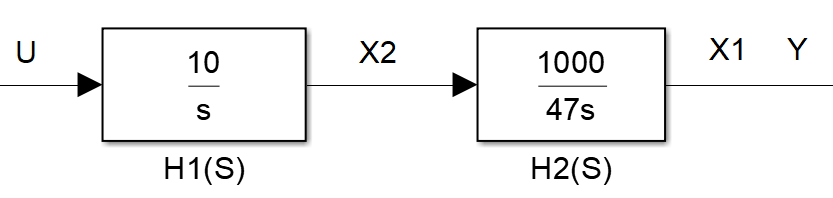
\includegraphics[width=0.7\linewidth]{Imagenes/HLazoAbierto.png}
\caption{Transferencia del sistema a lazo abierto}
\label{fig:diagramaOpen}
\end{figure}

Donde la transferencia de la planta a lazo abierto:
\[
G_P(S) = \frac{10}{S} \cdot \frac{1000}{47 \cdot S}
\]
Siendo $X_1$ y $X_2$ las variables de estado. Planteando las transferencias intermedias se obtienen las ecuaciones de estado:
\[
\frac{X_2}{U} = \frac{10}{S} \Longrightarrow \dot{x_2} = 10u
\]

\[
\frac{X_1}{X_2} = \frac{1000}{47 \cdot S} \Longrightarrow \dot{x_1} = \frac{1000}{47} \cdot x_2
\]
La ecuación de salida:

\[
y = x_1
\]

Armando el espacio de estados matricial se tiene:

\[
\begin{bmatrix}
\dot{x_1} \\
\dot{x_2} 
\end{bmatrix}
=
\begin{bmatrix}
0 & \frac{1000}{47} \\
0 & 0 
\end{bmatrix}
\cdot
\begin{bmatrix}
x_1 \\
x_2 
\end{bmatrix}
+
\begin{bmatrix}
0 \\
10 
\end{bmatrix}
\cdot
\begin{bmatrix}
u
\end{bmatrix}
\]

\[
\begin{bmatrix}
y
\end{bmatrix}
=
\begin{bmatrix}
1 & 0 
\end{bmatrix}
\cdot
\begin{bmatrix}
x_1 \\
x_2 
\end{bmatrix}
\]

\subsection{Análisis de controlabilidad}
Antes de poder efectuar la realimentación de estados, se analiza la controlabilidad del sistema:

\[
C_m
=
\begin{bmatrix}
B & AB
\end{bmatrix}
=
\begin{bmatrix}
0 & \frac{10000}{47} \\
10 & 0 
\end{bmatrix}
\Longrightarrow
\begin{vmatrix}
0 & \frac{10000}{47} \\
10 & 0 
\end{vmatrix}
=
-\frac{100000}{47}
\not=
0
\]

Y se verifica que el rango de la matriz es 2, por lo que el sistema es totalmente controlable.
A partir de la ecuación característica consierando la realimentación:

\[
\begin{vmatrix}
SI-A+BK
\end{vmatrix}
=0
\]

\[
\begin{bmatrix}
S & 0 \\
0 & S
\end{bmatrix}
-
\begin{bmatrix}
0 & \frac{1000}{47} \\
0 & 0
\end{bmatrix}
+
\begin{bmatrix}
0 & 0 \\
10k_1 & 10k_2
\end{bmatrix}
=
\begin{bmatrix}
S & -\frac{1000}{47} \\
10k_1 & S+10k_2
\end{bmatrix}
\Longrightarrow
\begin{vmatrix}
S & -\frac{1000}{47} \\
10k_1 & S+10k_2
\end{vmatrix}
=0
\]

\[
S^2 + 10k_2 \cdot S + \frac{10000}{47}k_1 = 0
\]

\newpage
\section{Diseño de realimentación lineal}
Se quiere aplicar realimentación lineal de estados de tal manera que el sistema a lazo cerrado tenga un $OS\% \leq 20\%$. Con dicho parámetro se calcula el amortiguamiento que tendrá el sistema realimentado:

\[
\xi = \frac{-ln(OS\% / 100)}{\sqrt{\pi^2 + ln^2(OS\% / 100)}} = 0.4559 < 1 \Longrightarrow \textrm{Régimen Subamortiguado}
\]



Aplicando la realimentación lineal de estados, el sistema adopta el formato siguiente:

\begin{figure}[H]
\centering
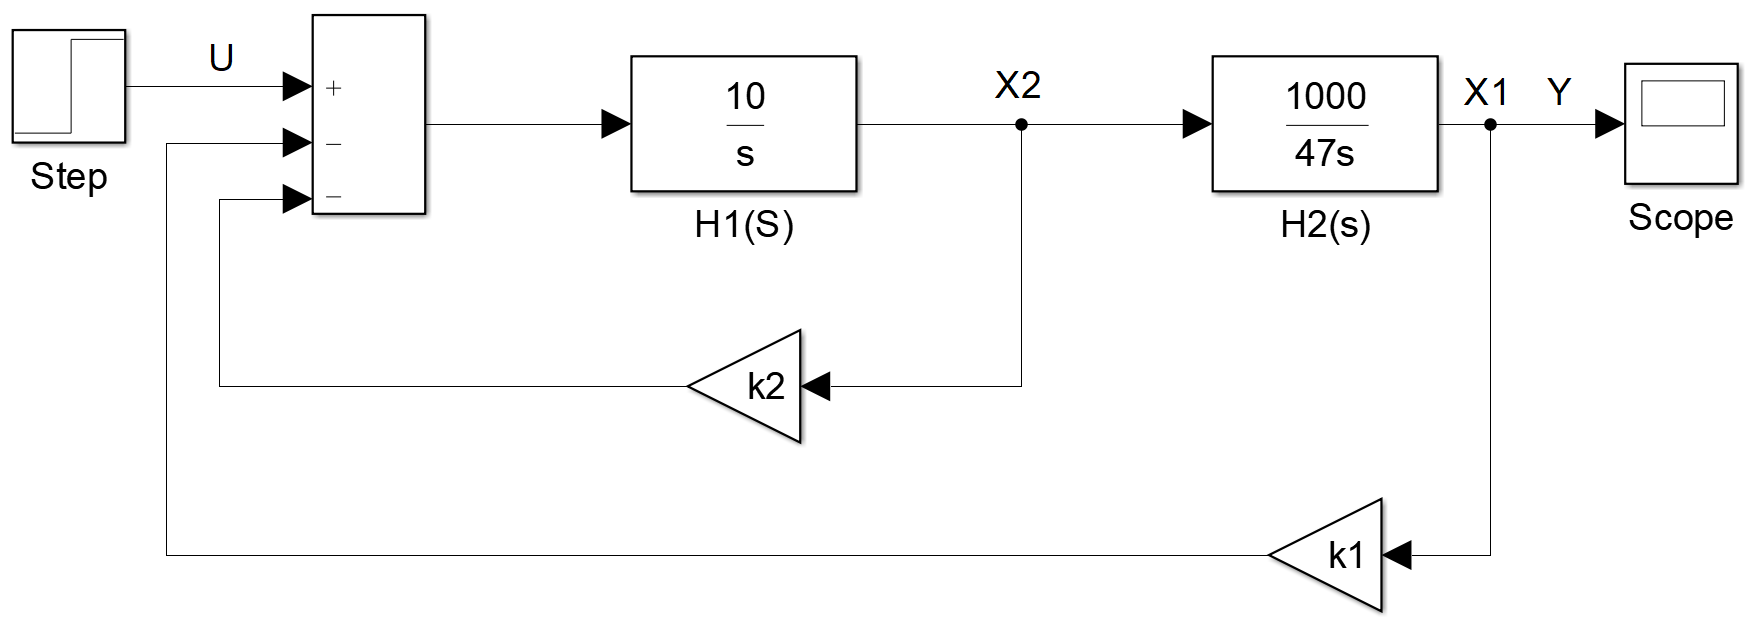
\includegraphics[width=0.9\linewidth]{Imagenes/HLazoCerrado.png}
\caption{Sistema realimentado}
\label{fig:diagramaClose}
\end{figure}

Donde la transferencia $T(S)$ en función de $k_1$ y $k_2$ resulta:

\[
T(S) = \frac{\frac{1000}{47}}{S^2 + 10k_2 \cdot S + \frac{10000}{47}k_1}
\]

Dado que se busca también que la ganancia del sistema a lazo cerrado (numerador) sea igual al término independiente del polinomio característico (denominador), resulta $k_1 = 1$. De esta forma se tiene que:

\[
\xi = 0.4559 \hspace{2cm} \omega_n^2 = \frac{10000}{47}
\]

Se sabe además que el término que acompaña a S en el polinomio de segundo orden es $2 \xi \omega_n$, por lo que igualando resulta:

\[
2 \xi \omega_n = 10k_2 \Longrightarrow k_2 = 1.34
\]

Finalmente, la transferencia del sistema a lazo cerrador resulta:

\[
T(S) = \frac{\frac{1000}{47}}{S^2 + 13.4 \cdot S + \frac{10000}{47}}
\]

\section{Implementación - Caso $k_2$ = 1.4}

Para implementar la realimentación, se agregan dos resistencias que den las ganancias $k_1$ y $k_2$ buscadas, siguiendo la configuración del operacional inversor:

\[
A_v = -\frac{10K\Omega}{R_k} 
\] 

Para obtener $k_1$, se utiliza $R_{k_1} = 10K\Omega$, y para obtener $k_2$ se utiliza $R_{k_2} = 6.8K\Omega + 330\Omega$ (en serie, de manera de acercarse lo más posible al valor de $k_2$ calculado).

\newpage

Agregando dichas resitencias, el circuito propuesto queda de la siguiente forma:

\begin{figure}[H]
\centering
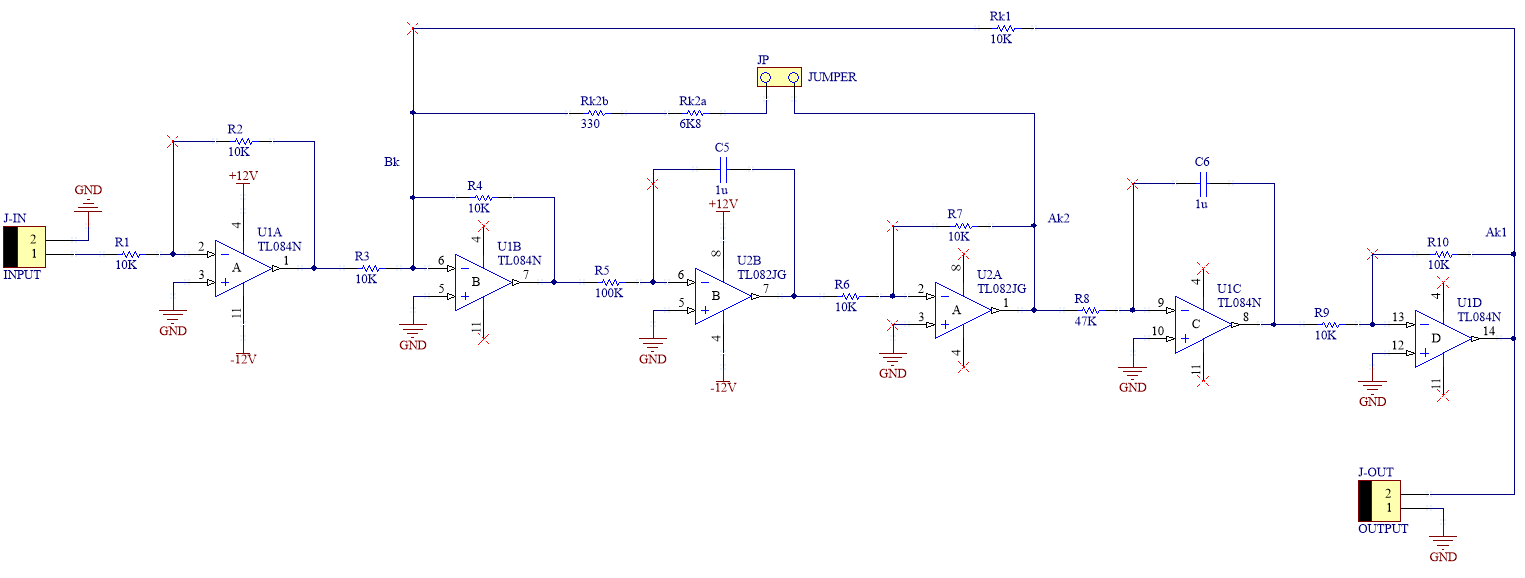
\includegraphics[width=1\linewidth]{Imagenes/CircuitoRealimentado.png}
\caption{Circuito realimentado}
\label{fig:Circuito}
\end{figure}

Los puntos de donde parten las resistencias $R_k$ ($A_{k_1}$ y $A_{k_2}$) respecto de la entrada no están invertidos en fase (dado que hay un número par de etapas inversoras de por medio), por lo que se conecta la realimentación al punto indicado ($B_k$), ya que respecto de la entrada esta invertido, por lo que actúa como restador.

\subsection{Simulación y Medición - Comparativa}

\subsubsection{Respuesta al escalón}

\begin{figure}[H]
\centering
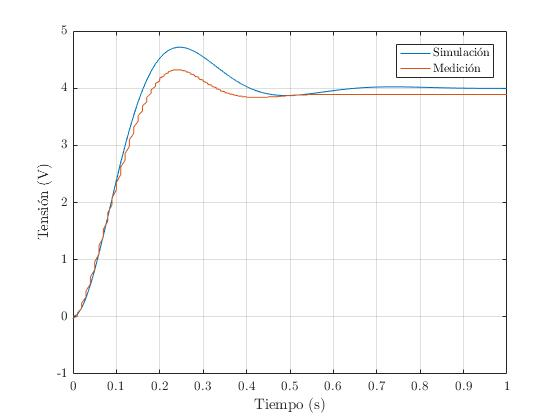
\includegraphics[width=0.8\linewidth]{../graficos/escalon1.jpg}
\caption{Respuesta al escalón - Caso $k_2$ = 1.4}
\label{fig:escalonNormal}
\end{figure}

De las respuestas obtenidas, tanto para el caso simulado como el medido se obtuvo un sobrepico porcentual menor al 20\% como se esperaba. En el caso medido fue de aproximadamente 10\%.
En la simulación, al ser bloques ideales puede notarse que el error permanente estacionario es nulo, tomando como valor final los 4V del escalón de entrada. En cambio, en el circuito medido, debido a las perturbaciones externas el sistema no llega completamente al valor esperado de 4V y posee un cierto error permanente de 0.2V (dado que llegaba hasta 3.8V). Dado el caso, la implementación real del sistema requeriría aplicar control integral si se busca tener un error permanente nulo.

\subsubsection{Plano de fase}

\begin{figure}[H]
\centering
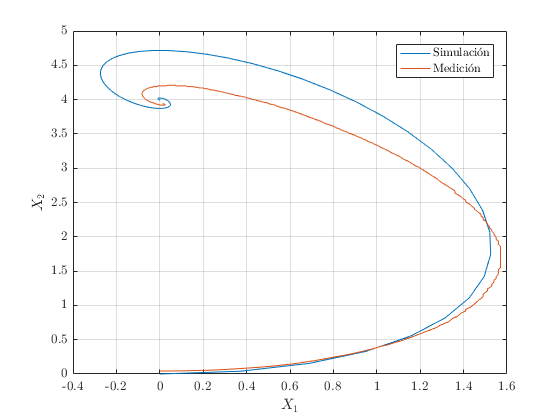
\includegraphics[width=0.8\linewidth]{../graficos-xy/xy.png}
\caption{Plano de fase - Caso $k_2$ = 1.4}
\label{fig:escalonNormal}
\end{figure}

De los gráficos obtenidos se observa que se corresponden efectivamente con la respuesta de un sistema subamortiguado, dada la forma espiralada. Ésta circula cerrándose hasta finalizar en un punto, verificando que el sistema es estable.

\section{Implementación - Caso con $k_2 = 0$}

En este caso se toma la transferencia genérica obtenida a lazo cerrado en función de $k_1$ y $k_2$, haciendo $k_2 = 0$ que equivale a abrir el camino del lazo que forma. La transferencia resilta entonces:

\[
T(S) = \frac{\frac{1000}{47}}{S^2 + \frac{10000}{47}}
\]

Dicha transferencia corresponde a una respuesta senoidal, por lo que se espera obtener luego en la simulación y mediciones una respuesta de dicha índole frente al escalón como entrada.

\subsection{Simulación y Medición - Comparativa}

\subsubsection{Respuesta al escalón}

\begin{figure}[H]
\centering
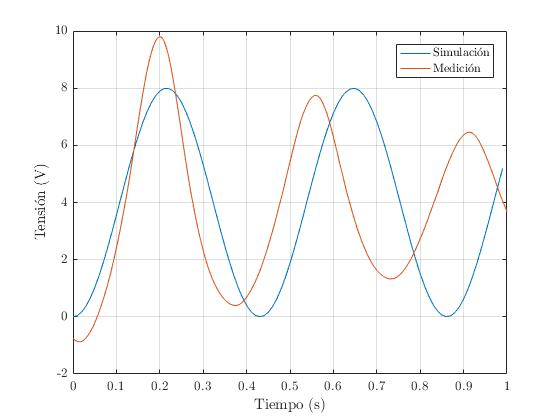
\includegraphics[width=0.8\linewidth]{../graficos/escalonSinK2.jpg}
\caption{Respuesta al escalón - Caso $k_2$ = 0}
\label{fig:escalonSinK2}
\end{figure}

De los gráficos obtenidos, como se esperaba en la simulación frente a la entrada escalón el sistema entra en un régimen oscilatorio, cuya frecuencia corresponde a $\omega_n$:

\[
\omega_n = \sqrt{\frac{10000}{47}} \Longrightarrow T_{OSC} = \frac{2 \pi}{\omega_n} = \textrm{0.43 seg.}
\]

En la señal medida, se observa también que el sistema comienza a oscilar, pero dada la no idealidad de los operacionales y los componentes, esta presenta una atenuación a lo largo del tiempo (como resulta visible en la gráfica mostrada) no llegando nunca a establecerse a un valor final.

\subsubsection{Plano de fase}

\begin{figure}[H]
\centering
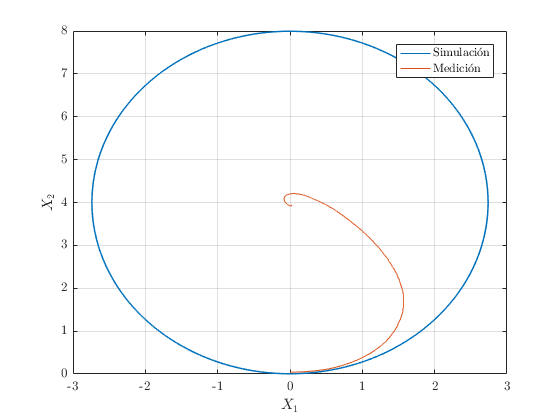
\includegraphics[width=0.8\linewidth]{../graficos-xy/xy-sin-k.png}
\caption{Respuesta al escalón - Caso $k_2$ = 0}
\label{fig:escalonSinK2}
\end{figure}

De los planos obtenidos, se observa que en el caso simulado, como es una oscilación ideal el gráfico resulta ser una circunferencia sin desviaciones. Por el otro lado, en el caso medido al ir atenuándose, el plano sigue la forma de espiral cerrándose, pero nunca llega a establecerse como se mencionó en la respuesta al escalón.

\end{document}
